\documentclass[tikz]{standalone}
\usepackage{amsmath}
\usetikzlibrary{positioning, matrix, shadows, shapes}

\thispagestyle{empty}
\begin{document}
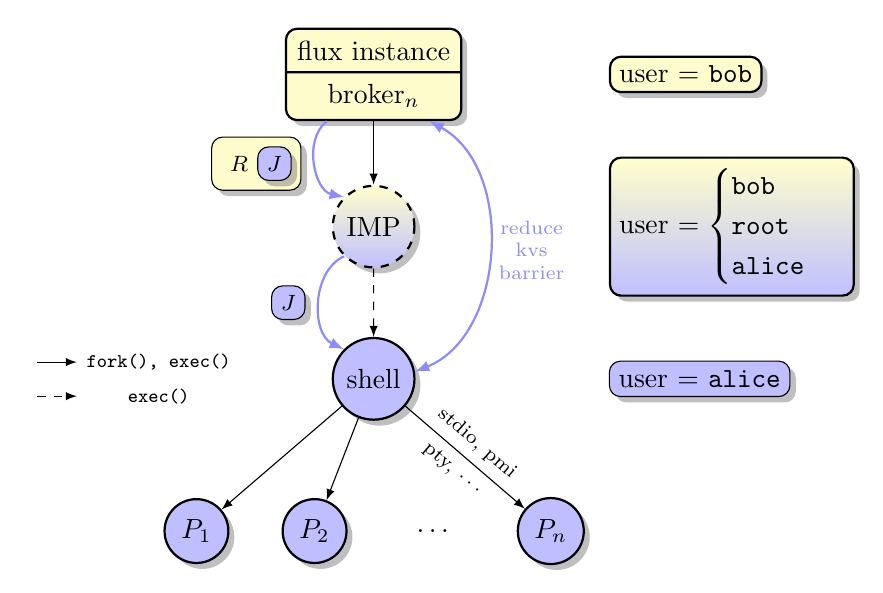
\begin{tikzpicture}[%
  node distance = 8.5em,
  broker/.style = {rectangle split, rectangle split parts = 2,
                   inner sep = .4em,
                   rounded corners, draw, thick,
                   align=center, fill=yellow!20, drop shadow},
  owner/.style =  {rectangle, rounded corners, draw, thick, fill=yellow!20,
                   drop shadow},
  proc/.style =   {circle, draw, thick, align=center, drop shadow,
                   fill=blue!25},
  IMP/.style =    {circle, draw, thick, dashed, align=center, drop shadow,
                   bottom color=blue!25, top color=yellow!20},
  impu/.style =   {rectangle, rounded corners, draw, thick, align=center,
                   bottom color=blue!25, top color=yellow!20, drop shadow},
  jtok/.style =   {rectangle, rounded corners, draw, align=center,
                   fill=blue!25, font=\footnotesize, drop shadow},
  user/.style =   {rectangle, rounded corners, draw, align=center,
                   fill=blue!25, drop shadow},
  rtok/.style =   {rectangle, rounded corners, draw, align=center,
                   fill=yellow!20, font=\footnotesize, drop shadow}
]


  \node[broker] (B) {flux instance \nodepart{second} broker$_n$}
    child[level distance=5.5em] {%
          node[IMP] (imp) {IMP}
          edge from parent[-latex]
          child {
                  node[proc] (sh) {shell}
                  edge from parent[dashed]
                  child[solid] {node[proc] (p1) {$P_1$} }
                  child[solid] {node[proc] (p2) {$P_2$} }
                  child {node[draw=none] {$\ldots$}
		    edge from parent[draw=none]
                  }
                  child[solid] {node[proc] (pn) {$P_n$} }
                }
           };

    % data flows
    \draw[-latex, thick, color=blue!45] (B.225)
                   to[in=220, out=135, bend right=65]
                    coordinate (step1)
                  (imp.135);
    \draw[-latex, thick, color=blue!45] (imp.225)
                  to[in=220, out=135, bend right=65]
                    coordinate (step2)
                  (sh.135);

    \node[rtok, matrix=true, left of=step1, anchor=east, node distance=.5em] {%
	 \node {$R$}; & \node[jtok] {$J$}; \\
         };
    \node[jtok, left of=step2, anchor=east, node distance=.5em] (J) {$J$};


    % legend

    \node [matrix, left of=sh, font=\scriptsize](legend)
    {
       \draw[-latex] (0,0) -- (.5,0);  & \node[] {\tt fork(), exec()}; \\
       \draw[-latex, dashed] (0,0) -- (.5,0); & \node[] {\tt exec()}; \\
    };

    % Annotations
    \node [align=left]  (bu) [owner, right of=B, anchor=west] {user = \tt bob};
    \node [align=left]  (su) [user, right of=sh, anchor=west] {user = \tt alice};
    \node [align=left]  (iu) [impu, right of=imp, anchor=west] {%
                               user $= \begin{cases}
                                          \tt bob \\
                                          \tt root \\
                                          \tt alice \\
                                        \end{cases}$
                               };

    % Connections
    \draw[<->,>=latex,color=blue!45,thick] (sh.10)
                   to[in=320, out=-50, bend right=65]
		   node[right, align=center,font=\scriptsize]
                        {reduce \\ kvs \\ barrier}
                  (B.320);

    %\path[] (sh) -- node [pnote, near end]    {stdio} (pn);
    %\path[] (sh) -- node [pnote, midway]      {pmi} (pn);
    %\path[] (sh) -- node [pnote, near start]  {pty} (pn);
    %\path[] (sh) -- node [pnote, very near end]  {$\ldots$}(pn) ;
    \path[] (sh) --
                 node [align=center, sloped, above, font=\scriptsize]
                      {stdio, pmi} (pn);
    \path[] (sh) --
                 node [align=center, sloped, below, font=\scriptsize]
                      {pty, $\cdots$} (pn);
	

\end{tikzpicture}
\end{document}
